\section{Future Research}
\label{sec:future}

\subsection{Chaotic Analytic Function Generation}

To illustrate the difference in the requirements on $\mathbf{J}$ and $f(x,y)$,
we employ a random analytic function generation technique as
described by Hannay \cite{hannay} and discussed earlier in the literature
section. \Cref{fig:caf} shows a preliminary plot of the isotropic, stationary
random analytic function generated using this method. Future research intends to
extend this to calculating the associated probability current, and compare it
with a generated divergenceless current.

In other words, the scalar function $\chi$ is randomly generated, and
$\mathbf{J}$ is calculated as
\begin{align}
    \mathbf{J} = \basis{z} \times \nabla \chi.
\end{align}
This should illustrate the difference between the ``typical'' probability
currents generated from the chaotic analytic $f(x,y)$ and from the scalar field
$\chi$ and confirm that analyticity is more stringent than divergencelessness.

\begin{figure}
    \centering
    \begin{minipage}{0.45\linewidth}
        \centering
        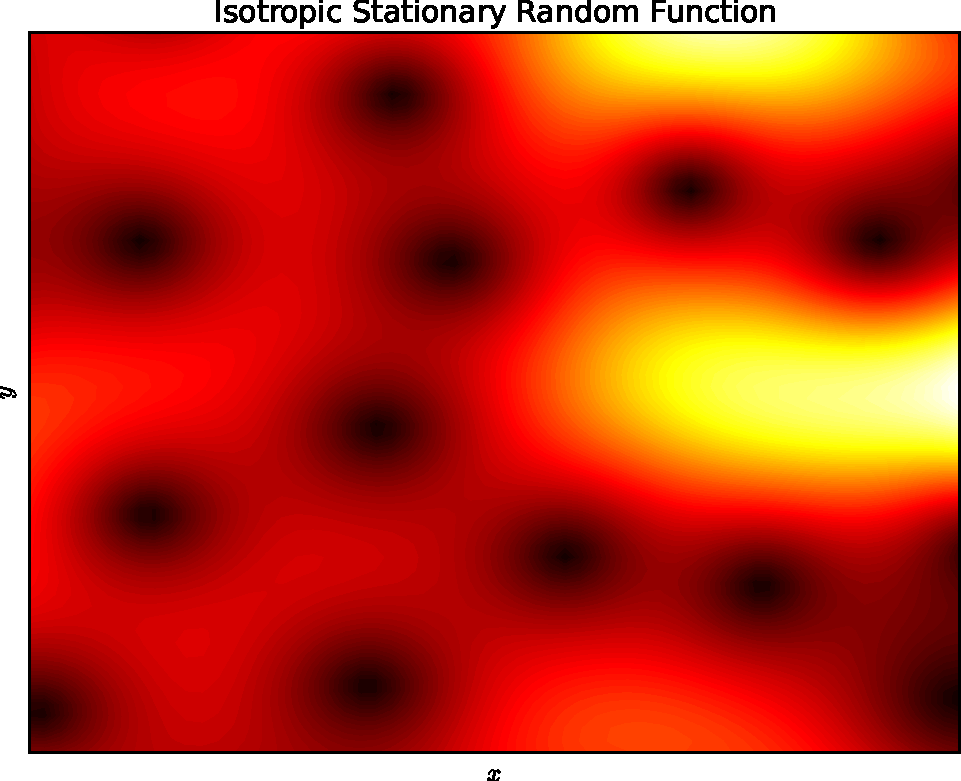
\includegraphics[width=\linewidth]{caf}
        \caption{The isotropic stationary function calculated from the generated
            chaotic analytic function. Note the presence of dark spots; the
            associated probability current should flow anticlockwise around these local
            minima.}
        \label{fig:caf}
    \end{minipage}
    \begin{minipage}{0.45\linewidth}
        \centering
        \def\svgwidth{\linewidth}
        \input{figures/magnetic-ab.pdf_tex}
        \caption{An illustration of the magnetic Aharonov-Bohm (AB) setup, where an
            infinitely long and thin solenoid causes the wavefunction overlap after
            a double slit to be non-simply connected, or have islands.}
        \label{fig:magnetic-ab}
    \end{minipage}
\end{figure}

\subsection{The Aharonov-Bohm Effect}

The Aharonov-Bohm (AB) effect shows that the electromagnetic potentials have an
effect on the wavefunction of a quantum system, even when the fields are zero
\cite{aharonov-bohm}.

For the magnetic case (as we will consider here), this amounts to $\mathbf{A}$
affecting the wavefunction independent of the choice of gauge, without any
magnetic field in the region of the wavefunction. This is often physically
explained as an infinitely long solenoid sitting behind a double slit, causing
non-simply connectedness in the overlapping wavefunctions
\cite{aharonov-rohrlich}, as shown in \Cref{fig:magnetic-ab}.  Although the
magnetic field is zero outside of the infinitely thin solenoid, the magnetic
vector potential is not, and it is this that causes a phase shift, as observed
on the screen.

Thus, although the ultimate effect is gauge independent (as it must be as it is
observable), the vector potential is seemingly \textit{requried} in the
prediction of the phase shift. Specifically, the phase difference between the
two wavefunctions is
\begin{align}
    \Delta \phi = e^{i q \Phi_B / \hbar},
\end{align}
where $\Phi_B = \oint \mathbf{A} \cdot d\mathbf{x}$ is the flux of the vector
potential around the cylinder \cite{aharonov-rohrlich}.

Further investigation will be carried out concerning the AB effect and the
supposed reliance on the gauge dependent potentials, with particular emphasis on
the possibility of additional freedoms.

\subsection{The Density Matrix}

Another topic of future investigation is the gauge freedom involved with the
density operator, $\hat \varrho$, given by
\begin{align}
    \varrho = \sum_i p_i \Ket{\psi_i}\bra{\psi_i},
\end{align}
where $p_i$ are the probabilities of the system being in state $\Ket{\psi_i}$,
and the sum is over all possible states such that $\sum_i p_i = 1$.

The density operator is gauge invariant. An interesting question, then, is
whether quantum mechanics can be recast in an entirely gauge invariant way using
this density operator formalism. In particular, the time evolution of the
density operator is given by its commutator with the Hamiltonian;
\begin{align}
    i \hbar \dot{\varrho} = \comm{H}{\varrho}.
\end{align}

This means that although the density operator is gauge independent, its time
evolution is generated by the gauge dependent Hamiltonian
\begin{align}
    H &= \frac{1}{2m} \mathbf{\Pi}^2 + qV \\
      &= \frac{1}{2m} \left( \mathbf{p} - q \mathbf{A} \right)^2 + qV.
\end{align}

Future research aims to investigate the degree to which we can circumvent this
gauge dependence, and express such phenomena entirely gauge independently.

\subsection{The Wigner Function}

Another interesting future line of inquest concerns the phase space equivalent
of the density operator: the Wigner function $W(x,p)$. This distribution is
defined in the position representation by
\begin{align}
    W(x,p) &\defeq \frac{1}{\pi \hbar} \int_{-\infty}^{\infty} \psi^*(x+y)
    \psi(x-y) e^{\frac{2ipy}{\hbar}} dy \\
    &= \frac{1}{\pi \hbar} \int_{-\infty}^{\infty} \varrho(x-y,x+y)
    e^{\frac{2ipy}{\hbar}} dy,
\end{align}
where $y$ is simply the half the difference between two points $x - y$ and $x +
y$ \cite{wigner}. In other words, (ignoring constants) the Wigner distribution is the Fourier
transform of the density operator in the position basis, $\varrho(x-y,x+y)$,
with respect to the difference between the two positions.

The time evolution of a Wigner function varying with time is given by the Moyal
equation:
\begin{align}
    \dot W(x,p) = \moyal{H(x,p)}{W(x,p)},
\end{align}
where $\moyal{A}{B}$ is the Moyal bracket of $A$ and $B$ and $H(x,p)$ is the
Hamiltonian on the phase space \cite{moyal}. The Moyal bracket is the phase space version of
the commutator;
\begin{align}
    \moyal{f}{g} &\defeq \frac{1}{i \hbar}\left( f \star g - g \star f \right)
    \\
    &= \poiss{f}{g} + O\left(\hbar^2\right),
\end{align}
where $f \star g$ is the Moyal product \cite{moyal},
\begin{align}
    f \star g \defeq fe^{\frac{i \hbar}{2} \left( \overleftarrow \partial_x
        \overrightarrow \partial_p - \overleftarrow \partial_p
        \overrightarrow \partial_x \right)} g.
\end{align}
Note that the direction of the arrow indicates the direction the partial
differentiation acts on; $u \overleftarrow \partial v = \left( \partial u\right)
v$ and $u \overrightarrow \partial v = u \left( \partial v \right)$.
\begin{align}
    \moyal{f}{g} = \poiss{f}{g} + O \left( \hbar^2 \right),
\end{align}
where $\poiss{f}{g}$ is the classical Poisson bracket
\begin{align}
    \poiss{f}{g} = f \left( \overleftarrow \partial_x \overrightarrow \partial_p
    - \overleftarrow \partial_p \overrightarrow \partial_x \right)  g.
\end{align}

Thus, taking $\lim_{\hbar \rightarrow 0}$, the Moyal equation becomes the
classical Liouville equation \cite[Page 27]{curtright-fairlie-zachos},
\begin{align}
    \dot P(x,p) = \poiss{H(x,p)}{P(x,p)},
\end{align}
where $P(x,p)$ is the classical probability distribution over phase space.

Although Wigner can be negative and is thus a $\textit{quasi}$-probability
distribution \cite[Page 8]{curtright-fairlie-zachos}, it provides a correspondence to
classical physics which could be of interest in the exploration of quantum gauge
circumvention; classically the gauge dependent potentials are useful but are not
needed in the same way that quantum seemingly needs it (as in the Aharonov-Bohm
case) \cite{aharonov-bohm}.
